\section{Methods}

\begin{figure*}[t]
  \centering
  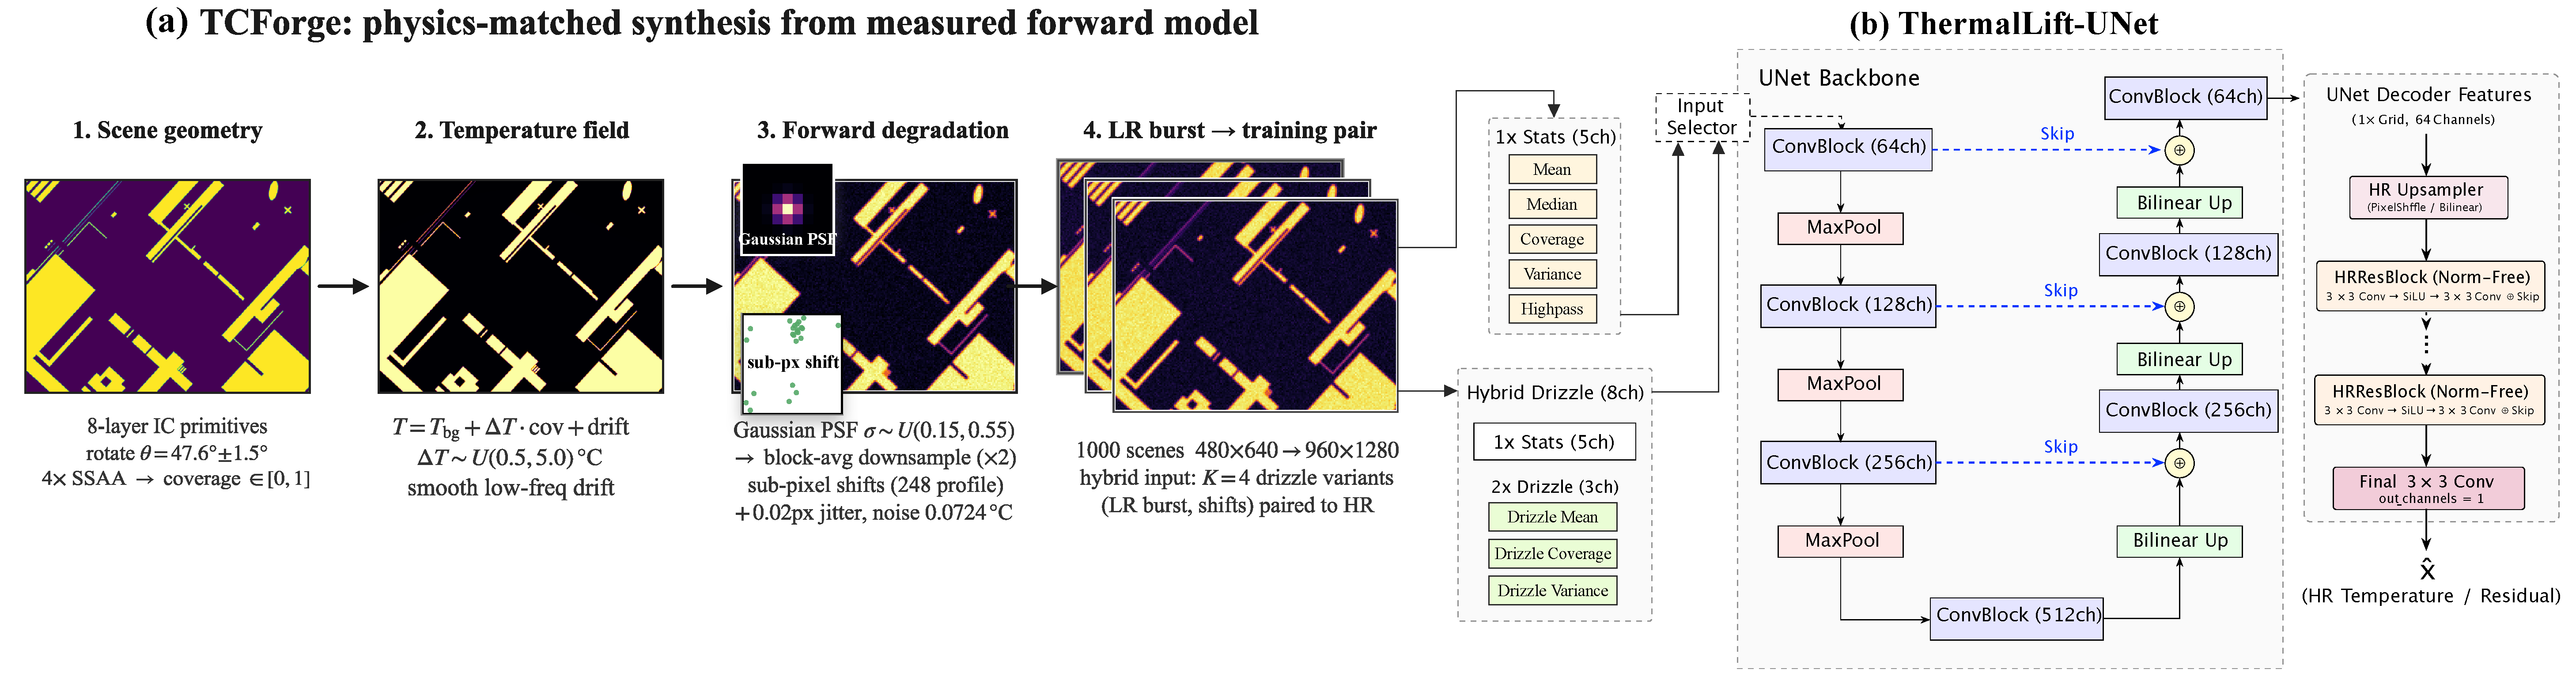
\includegraphics[width=\textwidth]{../figures/fig_tcforge_pipeline.pdf}
  \caption{Method overview: TCForge physics-matched synthesis pipeline, ThermalLift-UNet with two input modes, contour-oriented loss with observation-anchoring variants, and proxy-Pareto checkpoint selection.}
  \label{fig:method}
\end{figure*}

\subsection{Method Overview}

Our method has three components. First, we use three classical reconstruction methods as acceptance gates: a learning method is accepted only if it is not worse than the classical baseline on both FRC-band consistency and zigzag-profile metrics defined in Sec.~3.3 (acceptance rule in Appendix~C.5). Second, we build TCForge, a physics-matched synthetic training platform whose parameters all come from measurements, so learning is trained in synthetic domain and deployed in real domain. Third, under a fixed backbone, we vary input information pathways and observation anchoring, forming
\[
\{\text{1x stats},\ \text{hybrid drizzle}\}\times\{\text{none},\ \text{band},\ \text{full},\ \text{legal}\},
\]
to isolate how sub-pixel phase evidence delivery and loss-side anchoring constrain null-space drift.

\subsection{Classical Reconstruction Baselines}

\paragraph{Drizzle.}
After contour-refined alignment of all 248 frames, we project onto a $2\times$ grid via flux-conserving sub-pixel scatter \citep{fruchter2002drizzle} (pixfrac $=0.7$, square kernel), and set pixels with coverage $<1.0$ to NaN. Drizzle is a minimal-assumption fusion baseline and exposes coverage/lattice artifacts that any fine-grid method must manage; on a $5\times$ diagnostic grid, the mean zero-coverage rate reaches $27\%$.

\paragraph{MAP-TV Deconvolution Baseline.}
We build the Sec.~3.1 forward model on all 248 frames (shift $\to$ Gaussian PSF $\to$ $10\,\ensuremath{\mu m}$ detector box $\to$ downsample), and optimize with GPU FISTA \citep{beck2009fast} plus smooth-TV gradients for 150 iterations. Parameters are scanned on $\sigma_{\mathrm{PSF}}\in\{0.2,0.3,0.4,0.5\}\,\mathrm{LR\;px}$ and $\lambda_{\mathrm{TV}}\in\{3\times10^{-4},10^{-3},3\times10^{-3}\}$; split-half proxy combination selects $\sigma=0.2$ and $\lambda=10^{-3}$. MAP-TV serves as an acceptance gate (Appendix~C.5): a learning method is adopted only if it is not worse on both FRC-band consistency and zigzag-profile metrics.

\paragraph{Anisotropic Coverage-Weighted TGV.}
Raster acquisition induces anisotropic data constraints (in-row X neighbors have gap 1, inter-row Y neighbors have gap about 16). Standard isotropic TGV \citep{bredies2010tgv} thus produces horizontal stripe artifacts. We adapt the TGV proximal operator inside outer-loop FISTA in two ways.

First, anisotropic dual projection. In the inner Chambolle--Pock solver \citep{chambolle2011firstorder}, the first-order dual ball is replaced by an ellipse:
\[
\{(a,b):(a/r_a)^2+(b/r_b)^2\le1\},\quad r_a=\alpha_1\cdot r_y,\ r_b=\alpha_1,\ r_y=1.5,
\]
which weakens regularization along Y relative to X to compensate for weaker Y-side data support.

Second, coverage-weighted data gradients. For each HR pixel, data-fidelity gradient is divided by precomputed frame coverage (bilinear splat + PSF adjoint), rather than uniformly by frame count $K$. This corrects stripe patterns caused by bilinear scatter concentrating weights on fixed HR rows. Together, these two modifications reduce artifact score from 3.870 to 0.695 ($-82\%$), and increase raw-control correlation from 0.902 to 0.916.

\subsection{Physics-Matched Synthetic Platform (TCForge)}

Training data are synthesized from a measured forward model rather than learned degradation distributions. The synthesis pipeline has four stages.

Scene geometry uses 8-layer random primitives to form IC-like layouts (blocks, bars, L-traces, frames, details, vias, and pins). Global rotation jitters around measured $\theta=47.6^\circ$ with $U(-1.5^\circ,+1.5^\circ)$. To remove staircase aliasing in HR targets, $4\times$ SSAA is enabled by default: render on a $4\times$ canvas after rotation, then apply $4\times4$ mean downsampling to obtain continuous coverage in $[0,1]$. Temperature fields are rendered as
\[
T=T_{\mathrm{bg}}+\Delta T\cdot\text{coverage}+A_{\mathrm{drift}}\cdot\text{smooth\_noise},
\]
where $\Delta T\sim U(0.5,5.0)\,^\circ\mathrm{C}$ spans measured contrast, $\sigma_{\mathrm{PSF}}\sim U(0.15,0.55)$ spans the credible interval (Appendix~A.5.2), and noise follows a lognormal distribution whose mean equals measured $0.0724\,^\circ\mathrm{C}$. Forward degradation is Gaussian PSF $\to$ blockwise bilinear mean downsampling (scale 2), with sub-pixel shift replay from measured contour-refined 248-frame profiles plus jitter $\sigma_j=0.02$ px.

The current training pool contains 1000 scenes ($480\times640 \to 960\times1280$). The hybrid-input pool additionally stores full LR bursts and precomputes $K=4$ drizzle variants: $k=0$ is canonical all-frame no-noise; $k=1\text{--}3$ keep 60--100\% of frames and add $N(0,0.05\,\text{px})$ shift noise. During training, deterministic variant-index sampling bakes frame subsets and shift augmentation into precomputation to avoid dataloader stalls (details in supp.~C.1).

\subsection{Learning Method Family}

To avoid exposing internal run IDs in the paper narrative, we denote the family as ThermalLift-UNet and use ablation-readable short names in the main text: Stats, Stats+HP-FC, Stats+Full-FC, Hybrid, Hybrid+Native-FC, and Hybrid+ResObs. Internal training IDs are retained only in supplementary reproducibility mappings.

\paragraph{Backbone Network.}
All learning variants share the same frozen backbone; only input pathway and observation anchoring vary. The backbone is a standard UNet \citep{ronneberger2015unet} with base channels $c=64$: encoder with 3 MaxPool stages + ConvBlock (each block: $2\times3\times3$ Conv + GroupNorm \citep{wu2018group} + SiLU + SE attention \citep{hu2018squeeze}), channels $c,2c,4c,8c$; decoder with bilinear upsampling + skip concatenation + ConvBlock. The default HR head is bilinear-upsample (scale) followed by $3\times3$ Conv. Ablation variant Stats+PixelShuffle also tests a PixelShuffle head \citep{shi2016realtime} with ICNR initialization \citep{aitken2017checkerboard}; it introduces stripe artifacts and consistently worse proxies, and is kept only as head-attribution control (Sec.~5.7).

\paragraph{Contour-Oriented Loss.}
The total loss is
\[
\mathcal{L}=w_m\mathcal{L}_{\mathrm{MSE}}+w_{hp}\mathcal{L}_{\mathrm{HP}}+w_e\mathcal{L}_{\mathrm{Edge}}+w_s(1-\mathrm{SSIM})+w_{gv}\mathcal{L}_{\mathrm{GV}}+w_{fm}\mathcal{L}_{\mathrm{FM}}+w_r\mathcal{L}_R.
\]
$\mathcal{L}_{\mathrm{HP}}=\|HP(\hat{x})-HP(x)\|_1$ is highpass structural loss, with $HP(x)=x-G_{\sigma=5}(x)$, multiplied by structure/thin/gap weight maps for key regions. $\mathcal{L}_{\mathrm{GV}}=\|g_{x,\hat{x}}-g_{x,x}\|_1+\|g_{y,\hat{x}}-g_{y,x}\|_1$ preserves full gradient-vector information and captures edge inflation/distortion not visible to magnitude-only edge losses. $\mathcal{L}_{\mathrm{FM}}$ is forward consistency (detailed in Sec.~4.4.4). $\mathcal{L}_R=\mathrm{mean}(|\hat{x}-x_{\mathrm{input}}|)$ is residual penalty used only in Hybrid+ResObs (Sec.~4.4.5).

The mainline uses a conservative frozen weight shell (from Stats onward): $w_m=0.3$, $w_{hp}=0.8$ (structure boost 2.0, thin boost 3.0, gap boost 2.0), $w_{gv}=0.15$, $w_s=0.15$, $w_e=0.05$. Ablation variant HotLoss uses a more aggressive shell ($w_{hp}=1.0$, structure boost 4.0) and is retained as drift-amplification reference. Full weight-evolution history is in supp.~C.2.

\paragraph{Input Modes.}
Input mode is the first factor of the ablation matrix.

\textbf{1$\times$ statistical input (baseline).}
On a $1\times$ grid, we build five channels from aligned mean / median / coverage / variance / highpass fused, then upsample to HR with scale $=2$. This is the conventional featurization route, but our ablation (Sec.~5.3) shows that it collapses burst sub-pixel phase information at input encoding stage.

\textbf{Hybrid drizzle input.}
On a $2\times$ grid, we combine two information sources: channels 0--4 are the above 1x statistics bilinearly upsampled to $2\times$, while channels 5--7 are drizzle mean / coverage / variance rendered directly on the $2\times$ grid. The network then runs at effective scale $=1$ on the $2\times$ grid. Sub-pixel evidence thus enters as direct data, not as an implicit prior the network must infer.

\paragraph{Observation-Anchoring Variants.}
Observation anchoring is the second factor of the ablation matrix. All anchoring variants share the same mechanism: reproject network prediction $\hat{x}$ through measured forward operator $A=D\cdot B\cdot H\cdot S$ from Sec.~3.1 into the $1\times$ observation domain, then compare with held $1\times$ observation $y_{\mathrm{obs}}$.

\begin{table}[t]
  \centering
  \small
  \begin{tabular}{@{}llll@{}}
    \toprule
    Variant & Representative method & Anchoring mode & Description \\
    \midrule
    none & Stats / Hybrid & $w_{fm}=0$ & No observation anchoring \\
    HP-FC & Stats+HP-FC & $w_{fm}=0.1$, highpass & Forward consistency only on highpass band \\
    Full-FC & Stats+Full-FC & $w_{fm}=0.1$, full-band & Forward consistency over full band \\
    Native-FC & Hybrid+Native-FC & $w_{fm}=0.1$, highpass & Under hybrid input, anchoring consumes a separately carried native $1\times$ aligned-mean patch, not upsampled hybrid channel-0 mean \\
    \bottomrule
  \end{tabular}
  \caption{Observation-anchoring variants in the ablation matrix.}
\end{table}

All filled variants in this matrix---Stats, Stats+HP-FC, Stats+Full-FC (1x input), and Hybrid, Hybrid+Native-FC (hybrid input)---are trained to 60K steps. Drift trajectories in Sec.~5.2 show nearly identical drift curves across all loss-side anchoring variants.

\paragraph{Residual-over-Observation Parameterization (Hybrid+ResObs).}
On top of hybrid input, we add output parameterization: the network predicts residual $\delta$, and final output is
\[
\hat{x}=x_{\mathrm{drizzle}}^{\mathrm{ch5}}+\delta,
\]
where $x_{\mathrm{drizzle}}^{\mathrm{ch5}}$ is the input drizzle-mean channel. An L1 residual penalty
\[
\mathcal{L}_R=w_r\cdot\mathrm{mean}(|\delta|)
\]
controls how far output can move from drizzle observation base. Weight $w_r$ is parameterized by $\lambda$; scanning $\lambda\in\{0.2,0.5,1.2,3.0\}$ selects a working point on a 3D fine-window proxy trade-off (fidelity / sharpness / grain). Sec.~5.1 reports results for $\lambda=1.2$ at 15K steps. Hybrid+ResObs makes the trade-off tunable, but the selected row is still a high-sharpness, lower-correlation, higher-artifact operating point.

\subsection{Checkpoint Selection Protocol}

Using training endpoints (the field default) makes each variant output its worst checkpoint, which is a direct consequence under null-space drift. Checkpoint selection is therefore part of the method, not post-processing.

For all evaluated checkpoints of each variant, we first normalize two proxies to $[0,1]$:
\[
a_{\mathrm{norm}}=\frac{\text{artifact}-\min}{\max-\min},\qquad
c_{\mathrm{norm}}=\frac{\max_{\mathrm{corr}}-\text{corr}}{\max_{\mathrm{corr}}-\min_{\mathrm{corr}}}.
\]
We then compute distance to ideal point $(0,0)$ as $d=\sqrt{a_{\mathrm{norm}}^2+c_{\mathrm{norm}}^2}$, select up to 3 candidates by ascending $d$ with 5K-window deduplication, and force-add the 60K endpoint as drift reference if absent. Rank-1 is the canonical candidate. Every candidate must pass visual gating on the temperature-domain triplet panel. Full procedure is provided in supp.~C.5.

